no\documentclass{article}

% Additional packages & macros
\usepackage[a4paper, margin=1in]{geometry}
\usepackage{fancyhdr}
\pagestyle{fancy}
\usepackage{minted}
\usepackage{xcolor}
\usemintedstyle{pastie}
\usepackage{booktabs}     % For cleaner tables (\toprule, \midrule, \bottomrule)
\usepackage{amsmath}      % General maths support
\usepackage{amssymb}      % Additional maths symbols
\usepackage{graphicx}     % If you're including any images
\usepackage{hyperref}     % For clickable links (if needed)
\usepackage{tikz}
\usetikzlibrary{positioning}


% Header and footer
% ! Unit name
\newcommand{\unitName}{CAB302 Software Development}
% ! Unit semester 
\newcommand{\unitTime}{Semester 2, 2025}
% ! Unit coordinator name
\newcommand{\unitCoordinator}{Unit Coordinator: Alessandro Soro}
% ! Document authors
\newcommand{\documentAuthors}{Monica Borg}

\fancyhead[L]{\unitName}
\fancyhead[R]{\leftmark}
\fancyfoot[C]{\thepage}

\date{}

\begin{document}
%
\begin{titlepage}
    \vspace*{\fill}
    \begin{center}
        \LARGE{\textbf{\unitName}} \\[0.1in]
        \normalsize{\unitTime} \\[0.2in]
        \normalsize\textit{\unitCoordinator} \\[0.2in]
        \documentAuthors
    \end{center}
    \vspace*{\fill}
    \thispagestyle{empty}
\end{titlepage}
\newpage
%
\tableofcontents
\newpage
%
\section{Object Oriented Programming with Java}

\subsection{Java}
Java is a high-level, class-based, object-oriented programming language that is platform-independent and widely used for developing applications across desktop, web, and mobile environments. It follows the syntax and structure of the C-family of languages, making it familiar to developers with experience in C or C\#.

Originally created in the 1990s at Sun Microsystems, Java was designed to be platform-independent and architecture-neutral, enabling code to run consistently across various systems (regardless of endianness\footnote{Endianness, in computing, refers to the order in which bytes within a word of digital data are stored in computer memory or transmitted over a network. It can be either big-endian (most significant byte first) or little-endian (least significant byte first)}). Java supports automatic garbage collection, offers robust memory management, and was developed with the internet in mind. Since becoming open source in 2006, it has served as the primary platform for Android development.

A basic Java program includes a class definition and a \texttt{main} method, which serves as the entry point for execution. For example, a program that prints \texttt{Hello, world!} to the console can be written as:

\begin{minted}[fontsize=\small, linenos, breaklines]{java}
public class HelloWorld {
    public static void main(String[] args) {
        System.out.println("Hello, world!");
    }
}
\end{minted}

\subsection{Primitive Data Types in Java}
Java provides a set of built-in primitive data types for representing simple values. These types are not objects and form the most basic elements for data representation and manipulation:

\begin{table}[h!]
\centering
\begin{tabular}{@{}lll@{}}
\toprule
\textbf{Type} & \textbf{Size} & \textbf{Description} \\
\midrule
\texttt{byte}   & 8-bit   & Signed two’s complement integer. Range: \texttt{-128} to \texttt{127} \\
\texttt{short}  & 16-bit  & Signed two’s complement integer. Range: \texttt{-32,768} to \texttt{32,767} \\
\texttt{int}    & 32-bit  & Signed two’s complement integer. Range: \texttt{-2,147,483,648} to \texttt{2,147,483,647} \\
\texttt{long}   & 64-bit  & Signed two’s complement integer. Range: \texttt{-9,223,372,036,854,775,808} \\
                &         & to \texttt{9,223,372,036,854,775,807} \\
\texttt{float}  & 32-bit  & IEEE 754 single-precision floating point \\
\texttt{double} & 64-bit  & IEEE 754 double-precision floating point \\
\texttt{boolean}& 1-bit*  & Represents \texttt{true} or \texttt{false} \\
\texttt{char}   & 16-bit  & A single Unicode character \\
\bottomrule
\end{tabular}
\end{table}
\textit{*Note: The size of a \texttt{boolean} is not fixed and depends on the JVM implementation. It is often 1 byte but not guaranteed.}

\subsection{Java Operators}

\subsubsection{Arithmetic Operators}
\begin{center}
\begin{tabular}{@{}lll@{}}
\toprule
\textbf{Operator} & \textbf{Name} & \textbf{Example} \\
\midrule
\texttt{+}  & Addition       & \texttt{x + y} \\
\texttt{-}  & Subtraction    & \texttt{x - y} \\
\texttt{*}  & Multiplication & \texttt{x * y} \\
\texttt{/}  & Division       & \texttt{x / y} \\
\texttt{\%} & Modulus        & \texttt{x \% y} \\
\texttt{++} & Increment      & \texttt{++x} \\
\texttt{--} & Decrement      & \texttt{--x} \\
\bottomrule
\end{tabular}
\end{center}

\vspace{1em}
\subsubsection{Assignment Operators}
\begin{center}
\begin{tabular}{@{}lll@{}}
\toprule
\textbf{Operator} & \textbf{Example} & \textbf{Equivalent To} \\
\midrule
\texttt{=}    & \texttt{x = 5}    & \texttt{x = 5} \\
\texttt{+=}   & \texttt{x += 3}   & \texttt{x = x + 3} \\
\texttt{-=}   & \texttt{x -= 3}   & \texttt{x = x - 3} \\
\texttt{*=}   & \texttt{x *= 3}   & \texttt{x = x * 3} \\
\texttt{/=}   & \texttt{x /= 3}   & \texttt{x = x / 3} \\
\texttt{\%=}  & \texttt{x \%= 3}  & \texttt{x = x \% 3} \\
\texttt{\&=}  & \texttt{x \&= 3}  & \texttt{x = x \& 3} \\
\texttt{|=}   & \texttt{x |= 3}   & \texttt{x = x | 3} \\
\texttt{\^=}  & \texttt{x \^= 3}  & \texttt{x = x \^ 3} \\
\texttt{>>=}  & \texttt{x >>= 3}  & \texttt{x = x >> 3} \\
\texttt{<<=}  & \texttt{x <<= 3}  & \texttt{x = x << 3} \\
\bottomrule
\end{tabular}
\end{center}

\vspace{1em}
\subsubsection{Logical Operators}
\begin{center}
\begin{tabular}{@{}lll@{}}
\toprule
\textbf{Operator} & \textbf{Name} & \textbf{Example} \\
\midrule
\texttt{\&\&} & Logical AND & \texttt{x < 5 \&\& x < 10} \\
\texttt{||}  & Logical OR  & \texttt{x < 5 || x < 4} \\
\texttt{!}   & Logical NOT & \texttt{!(x < 5 \&\& x < 10)} \\
\bottomrule
\end{tabular}
\end{center}

\vspace{1em}
\subsubsection{Comparison Operators}
\begin{center}
\begin{tabular}{@{}lll@{}}
\toprule
\textbf{Operator} & \textbf{Name} & \textbf{Example} \\
\midrule
\texttt{==} & Equal to                 & \texttt{x == y} \\
\texttt{!=} & Not equal                & \texttt{x != y} \\
\texttt{>}  & Greater than             & \texttt{x > y} \\
\texttt{<}  & Less than                & \texttt{x < y} \\
\texttt{>=} & Greater than or equal to & \texttt{x >= y} \\
\texttt{<=} & Less than or equal to    & \texttt{x <= y} \\
\bottomrule
\end{tabular}
\end{center}

\subsubsection{Operator Overloading}

Java does \textbf{not support operator overloading}. This means the behaviour of standard operators (e.g., \texttt{+}, \texttt{-}) cannot be redefined for user-defined types such as classes.

\subsection{Object-Oriented Principles in Java}

Java’s object-oriented paradigm is based on four core principles:

\begin{itemize}
    \item \textbf{Encapsulation} – Data (fields) and behaviour (methods) are combined into classes. Internal state is protected using access modifiers.
    \item \textbf{Abstraction} – Interface definitions and abstract classes allow internal implementation to be hidden while exposing only essential behaviour.
    \item \textbf{Inheritance} – A class can inherit from another to reuse properties and behaviour via the \texttt{extends} keyword.
    \item \textbf{Polymorphism} – Method behaviour can vary depending on the runtime object type, achieved via overriding and interfaces.
\end{itemize}

\subsubsection{Everything's an Object}

In Java, \texttt{java.lang.Object} is the ultimate superclass of all classes. Every Java object (including arrays) inherits its methods. These include:

\begin{itemize}
    \item \texttt{clone()} – Returns a copy of the object (shallow copy).
    \item \texttt{equals(Object obj)} – Compares for equality.
    \item \texttt{hashCode()} – Generates a hash code for use in hash tables.
    \item \texttt{toString()} – Returns a string representation of the object.
    \item \texttt{getClass()} – Provides the object's runtime class.
    \item \texttt{finalize()} – Invoked by the garbage collector before destruction.
    \item \texttt{wait()}, \texttt{notify()}, \texttt{notifyAll()} – Used for thread coordination.
\end{itemize}

These methods form the core behaviours available to every Java object.

\smallskip
\textit{See:} \href{https://docs.oracle.com/javase/8/docs/api/java/lang/Object.html}{\texttt{docs.oracle.com/javase/8/docs/api/java/lang/Object.html}}

\subsection{Foundational Java Features}

This section outlines core language features in Java that support structured program development and object-oriented design.

\subsubsection{Classes}

Classes serve as templates for defining objects, encapsulating both data and behaviour. Each class may define fields, methods, and constructors to manage its internal state and expose functionality.

\begin{minted}[fontsize=\small, linenos, breaklines]{java}
class Person {
    private String name;

    public Person(String name) {
        this.name = name;
    }

    public void greet() {
        System.out.println("Hello, " + name + "!");
    }
}
\end{minted}

While classes are fundamental to object-oriented design, \hyperref[subsec:interfaces]{interfaces} are often preferred when defining shared behaviour across unrelated types. Java supports only single inheritance for classes, meaning a class can extend only one superclass. In contrast, interfaces allow multiple inheritance of type, enabling a class to implement multiple interfaces. This promotes greater flexibility, modularity, and adherence to the principle of programming to an interface rather than to an implementation.



\subsubsection{Constructors and Encapsulation}

Constructors are used to initialise objects when they are created. Encapsulation ensures internal fields are kept private, with controlled access provided through methods (getters and setters).

\begin{minted}[fontsize=\small, linenos, breaklines]{java}
class BankAccount {
    private double balance;

    public BankAccount(double initialBalance) {
        balance = initialBalance;
    }

    public double getBalance() {
        return balance;
    }

    public void deposit(double amount) {
        if (amount > 0) {
            balance += amount;
        }
    }
}
\end{minted}

\subsubsection{Command Line Arguments}

Command line arguments are passed to Java applications through the \texttt{main} method. These values can be used to modify program behaviour at runtime.

\begin{minted}[fontsize=\small, linenos, breaklines]{java}
public class ArgumentPrinter {
    public static void main(String[] args) {
        if (args.length > 0) {
            System.out.println("First argument: " + args[0]);
        } else {
            System.out.println("No arguments provided.");
        }
    }
}
\end{minted}

\subsubsection{Standard Output}

Output to the console is typically performed using \texttt{System.out.print()} and \texttt{System.out.println()}. These are commonly used for program feedback and debugging.

\begin{minted}[fontsize=\small, linenos, breaklines]{java}
public class OutputExample {
    public static void main(String[] args) {
        System.out.print("This is printed on the same line. ");
        System.out.println("This ends with a newline.");
    }
}
\end{minted}


\subsection{Using Interfaces in Java for OOP}
\label{subsec:interfaces}

In Java, an \texttt{interface} defines a set of method signatures that implementing classes must fulfil. This promotes abstraction and allows different classes to share common behaviour without enforcing inheritance.

Interfaces may contain:
\begin{itemize}
    \item Abstract methods (implicitly \texttt{public abstract})
    \item \texttt{default} methods with implementation
    \item \texttt{static} methods
    \item Constants (\texttt{public static final})
\end{itemize}

Classes implement interfaces using the \texttt{implements} keyword. All abstract methods must be defined by the implementing class.

Interfaces are preferred in Java over class inheritance when designing for flexibility and modularity. Since Java does not support multiple class inheritance, interfaces offer a mechanism for multiple behavioural inheritance. This approach avoids the fragility associated with deep inheritance hierarchies and encourages composition over inheritance. It also enables different classes to share a common set of behaviours without enforcing a shared ancestry.


\subsubsection*{Example: Interface \& Implementation}

\begin{minted}[fontsize=\small, linenos, breaklines]{java}
interface Animal {
    void makeSound(); // abstract method
}

class Dog implements Animal {
    public void makeSound() {
        System.out.println("Woof!");
    }
}

class Cat implements Animal {
    public void makeSound() {
        System.out.println("Meow!");
    }
}

public class Main {
    public static void main(String[] args) {
        Animal a1 = new Dog();
        Animal a2 = new Cat();
        a1.makeSound(); // Woof!
        a2.makeSound(); // Meow!
    }
}
\end{minted}

This example demonstrates \textbf{polymorphism} through interface references. Both \texttt{Dog} and \texttt{Cat} implement \texttt{Animal}, enabling uniform handling while invoking class-specific behaviour.

\medskip
\textit{Interfaces are well suited for defining contracts that can be shared across unrelated classes.}

\subsection{Object-Oriented Libraries in Java}

The Java Standard Library includes a comprehensive collection of packages built on object-oriented principles. These libraries provide reusable classes for data structures, file I/O, networking, time manipulation, and system interaction.

\subsubsection*{java.util}

This package provides utility classes including collections, data structures, random number generation, and date/time classes.

\begin{itemize}
    \item \texttt{ArrayList} – A dynamically resizing array.
    \item \texttt{HashMap} – A key-value data structure with constant-time lookup.
    \item Additional utilities include \texttt{LinkedList}, \texttt{HashSet}, \texttt{Date}, \texttt{Calendar}, and \texttt{Random}.
\end{itemize}

\noindent\textbf{Example: Using \texttt{ArrayList} and \texttt{HashMap}}
\begin{minted}[fontsize=\small, linenos, breaklines]{java}
import java.util.ArrayList;
import java.util.HashMap;

public class UtilExample {
    public static void main(String[] args) {
        ArrayList<String> names = new ArrayList<>();
        names.add("Alice");
        names.add("Bob");

        HashMap<String, Integer> scores = new HashMap<>();
        scores.put("Alice", 85);
        scores.put("Bob", 90);

        System.out.println("Names: " + names);
        System.out.println("Bob's score: " + scores.get("Bob"));
    }
}
\end{minted}

\subsubsection*{java.io}

Provides classes for input/output streams, file access, character encoding, and buffered I/O operations.

\begin{itemize}
    \item \texttt{File}, \texttt{FileReader}, \texttt{FileWriter}
    \item \texttt{BufferedReader}, \texttt{PrintWriter}
    \item \texttt{InputStream}, \texttt{OutputStream}
\end{itemize}

\noindent\textbf{Example: Writing to and reading from a file}
\begin{minted}[fontsize=\small, linenos, breaklines]{java}
import java.io.*;

public class IOExample {
    public static void main(String[] args) throws IOException {
        // Write to file
        PrintWriter writer = new PrintWriter("example.txt");
        writer.println("Hello, file!");
        writer.close();

        // Read from file
        BufferedReader reader = new BufferedReader(new FileReader("example.txt"));
        String line = reader.readLine();
        System.out.println("Read: " + line);
        reader.close();
    }
}
\end{minted}

\subsubsection*{java.net}

This package enables network communication using sockets, IP addresses, and URLs.

\begin{itemize}
    \item \texttt{Socket}, \texttt{ServerSocket}
    \item \texttt{URL}, \texttt{URLConnection}
    \item \texttt{InetAddress}
\end{itemize}

\noindent\textbf{Example: Accessing a web page using \texttt{URL}}
\begin{minted}[fontsize=\small, linenos, breaklines]{java}
import java.net.*;
import java.io.*;

public class NetworkExample {
    public static void main(String[] args) throws Exception {
        URL url = new URL("https://example.com");
        BufferedReader reader = new BufferedReader(
            new InputStreamReader(url.openStream()));
        String line;
        while ((line = reader.readLine()) != null) {
            System.out.println(line);
        }
        reader.close();
    }
}
\end{minted}

\subsubsection*{java.lang}

Contains essential classes such as \texttt{Object}, \texttt{System}, \texttt{Math}, and wrapper types. It is automatically imported into every Java program.

\begin{itemize}
    \item \texttt{Object} – Superclass of all Java classes
    \item \texttt{System} – Access to standard input/output and system properties
    \item \texttt{Math}, \texttt{String}, \texttt{Integer}, etc.
\end{itemize}

\noindent\textbf{Example: Using \texttt{System} and \texttt{Math}}
\begin{minted}[fontsize=\small, linenos, breaklines]{java}
public class LangExample {
    public static void main(String[] args) {
        System.out.println("Square root of 64 is: " + Math.sqrt(64));
        System.out.println("Available memory: " + Runtime.getRuntime().freeMemory());
    }
}
\end{minted}

\subsubsection*{java.time}

Introduced in Java 8, this package provides a modern date and time API with immutable and thread-safe classes.

\begin{itemize}
    \item \texttt{LocalDate}, \texttt{LocalTime}, \texttt{LocalDateTime}
    \item \texttt{Duration}, \texttt{Period}, \texttt{ZoneId}, \texttt{ZonedDateTime}
    \item Preferred over \texttt{java.util.Date} and \texttt{Calendar} for new development
\end{itemize}

\noindent\textbf{Example: Working with dates and times}
\begin{minted}[fontsize=\small, linenos, breaklines]{java}
import java.time.LocalDate;
import java.time.LocalTime;
import java.time.LocalDateTime;

public class TimeExample {
    public static void main(String[] args) {
        LocalDate date = LocalDate.now();
        LocalTime time = LocalTime.now();
        LocalDateTime dateTime = LocalDateTime.now();

        System.out.println("Date: " + date);
        System.out.println("Time: " + time);
        System.out.println("DateTime: " + dateTime);
    }
}
\end{minted}

\subsubsection*{java.nio.file}

This package is part of the NIO.2 API and provides advanced file and directory handling with improved performance and flexibility.

\begin{itemize}
    \item \texttt{Files} – Static methods for file operations (e.g., copy, move, delete)
    \item \texttt{Paths}, \texttt{Path} – Represent file and directory locations
    \item Supports symbolic links, file attributes, and stream-based file access
\end{itemize}

\noindent\textbf{Example: Reading all lines from a file}
\begin{minted}[fontsize=\small, linenos, breaklines]{java}
import java.nio.file.*;
import java.io.IOException;
import java.util.List;

public class NioExample {
    public static void main(String[] args) throws IOException {
        Path path = Paths.get("example.txt");
        List<String> lines = Files.readAllLines(path);
        for (String line : lines) {
            System.out.println(line);
        }
    }
}
\end{minted}

\subsection{Git \& Version Control}

Version control is a fundamental practice in software development, particularly when collaborating in teams or managing large codebases. It provides a structured way to track, manage, and merge changes across multiple contributors and development branches.

\subsubsection{Why Version Control Is Necessary}

Collaborative coding efforts, especially in industry environments, require reliable systems for sharing and updating project files. Informal methods such as using USB drives or cloud file-sharing services (e.g., Google Drive) introduce several limitations:

\begin{itemize}
    \item Concurrency issues: Files cannot be safely edited by multiple contributors at the same time.
    \item Risk of loss or overwrite: Manual file sharing increases the likelihood of accidental data loss.
    \item No change tracking: It becomes difficult to determine what changes were made, by whom, and when.
\end{itemize}

To mitigate these issues, version control systems (VCS) are used universally in professional development workflows.

\subsubsection{What Is Version Control?}

Version control is a system that records changes to files over time, allowing earlier versions to be retrieved when needed. In addition to change tracking, version control provides essential features such as:

\begin{itemize}
    \item \textbf{Collaboration} – Enables concurrent development by multiple team members.
    \item \textbf{History tracking} – Maintains a complete, timestamped record of all modifications.
    \item \textbf{Branching and merging} – Allows isolated development of features or fixes, which can later be integrated into the main codebase.
\end{itemize}

\subsubsection{Types of Version Control Systems}

Version control systems can be broadly classified into three categories:

\begin{itemize}
    \item \textbf{Local Version Control Systems} – Store change history on a single machine (e.g., RCS).
    \item \textbf{Centralised Version Control Systems} – Use a single server to store all versions (e.g., Subversion).
    \item \textbf{Distributed Version Control Systems} – Each user has a complete local copy of the repository (e.g., Git, Mercurial).
\end{itemize}

\subsubsection{Version Control Tools and Adoption Rates}

Several tools implement version control with varying degrees of popularity:

\begin{itemize}
    \item \textbf{Git} – Used in over 70\% of projects; the most widely adopted distributed VCS.
    \item \textbf{Subversion (SVN)} – Centralised system, used in approximately 15\% of cases.
    \item \textbf{Perforce} – Popular in certain enterprise and game development contexts (< 5\%).
    \item \textbf{Mercurial} – Distributed system with similar capabilities to Git (< 5\%).
\end{itemize}


\subsubsection{Version Control Tools and Adoption Rates}

Several tools implement version control with varying degrees of popularity:

\begin{itemize}
    \item \textbf{Git} – Used in over 70\% of projects; the most widely adopted distributed VCS.
    \item \textbf{Subversion (SVN)} – Centralised system, used in approximately 15\% of cases.
    \item \textbf{Perforce} – Popular in certain enterprise and game development contexts (< 5\%).
    \item \textbf{Mercurial} – Distributed system with similar capabilities to Git (< 5\%).
\end{itemize}

\subsubsection{Git Overview}

Git is a distributed version control system developed by Linus Torvalds, the creator of the Linux kernel. It was specifically designed to manage large-scale software projects with speed and flexibility.

\textbf{Key goals of Git:}
\begin{itemize}
    \item High performance and efficiency
    \item Full support for non-linear development (branching and merging)
    \item Distributed architecture – every developer has a full copy of the repository
\end{itemize}

\subsubsection{Using Git}

Git can be used as a standalone system or integrated with hosting platforms that facilitate collaborative development. Common platforms that use Git include:

\begin{itemize}
    \item \textbf{GitHub}
    \item \textbf{GitLab}
    \item \textbf{Bitbucket}
    \item \textbf{Azure DevOps}
\end{itemize}

These platforms typically provide web interfaces, issue tracking, pull requests, and continuous integration pipelines built on top of the Git version control system.

\subsubsection{Visualisaion of a Git Repository}
\resizebox{\textwidth}{!}{
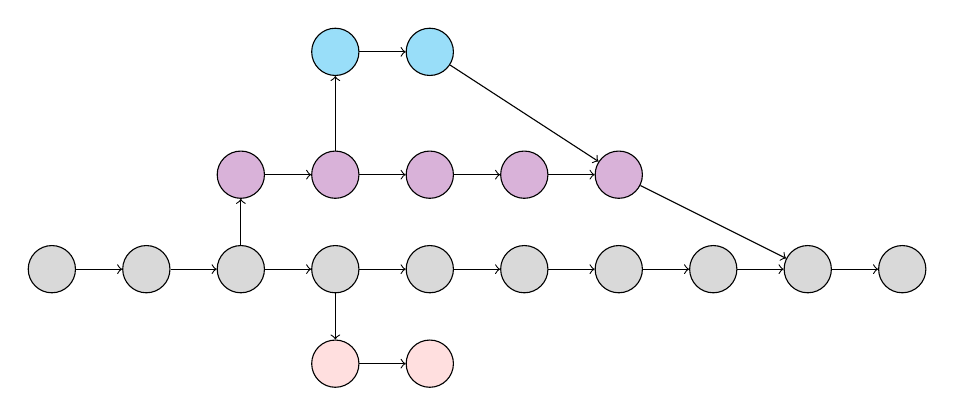
\begin{tikzpicture}[x=1.2cm, y=1.2cm, every node/.style={circle, draw, minimum size=6mm, inner sep=0pt}]

% Main branch nodes (10 total)
\foreach \x in {0,...,9}
    \node[fill=gray!30] (m\x) at (\x, 0) {};

% Edges for Main
\foreach \x in {0,...,8}
    \draw[->] (m\x) -- (m\the\numexpr\x+1\relax);

% Feature B (pastel pink)
\node[fill=pink!50] (b0) at (3, -1) {};
\node[fill=pink!50] (b1) at (4, -1) {};
\draw[->] (m3) -- (b0);
\draw[->] (b0) -- (b1);

% Feature A (pastel purple)
\node[fill=violet!30] (a0) at (2, 1) {};
\node[fill=violet!30] (a1) at (3, 1) {};
\node[fill=violet!30] (a2) at (4, 1) {};
\node[fill=violet!30] (a3) at (5, 1) {};
\node[fill=violet!30] (a4) at (6, 1) {};
\draw[->] (m2) -- (a0);
\draw[->] (a0) -- (a1);
\draw[->] (a1) -- (a2);
\draw[->] (a2) -- (a3);
\draw[->] (a3) -- (a4);
\draw[->] (a4) -- (m8);

% Feature A-1 (cornflower blue)
\node[fill=cyan!40] (a1a) at (3, 2.3) {};
\node[fill=cyan!40] (a1b) at (4, 2.3) {};
\draw[->] (a1) -- (a1a);
\draw[->] (a1a) -- (a1b);
\draw[->] (a1b) -- (a4);  % Merge into end of Feature A

\end{tikzpicture}
}

\vspace{1em}

\begin{center}
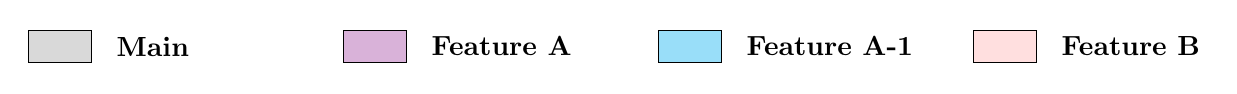
\begin{tikzpicture}[x=2cm, y=1cm]
    \draw[fill=gray!30]     (0,0) rectangle (0.4,0.4); \node[anchor=west] at (0.5,0.2) {\textbf{Main}};
    \draw[fill=violet!30]   (2,0) rectangle (2.4,0.4); \node[anchor=west] at (2.5,0.2) {\textbf{Feature A}};
    \draw[fill=cyan!40]     (4,0) rectangle (4.4,0.4); \node[anchor=west] at (4.5,0.2) {\textbf{Feature A-1}};
    \draw[fill=pink!50]     (6,0) rectangle (6.4,0.4); \node[anchor=west] at (6.5,0.2) {\textbf{Feature B}};
\end{tikzpicture}
\end{center}

\subsubsection{Local and Remote Repositories}

Version control in Git distinguishes between two primary types of repositories: local and remote. Understanding their relationship is fundamental to managing workflow and collaboration effectively.

\paragraph*{Local Repository}
A local repository exists on the developer's machine and includes the full history of commits, branches, and configuration files. It enables complete version control functionality without requiring a network connection.

\begin{itemize}
    \item Accessible only to the user of the local machine.
    \item Supports full Git operations such as commit, branch, revert, and diff.
    \item Local changes remain private until explicitly shared with others.
\end{itemize}

\paragraph*{Remote Repository}
A remote repository is hosted on an external server or cloud platform (e.g., GitHub, GitLab, Bitbucket). It serves as a shared version of the project that can be accessed by authorised collaborators.

\begin{itemize}
    \item Enables cloning, pushing, and pulling across distributed teams.
    \item Serves as a central copy for collaboration, backup, and integration.
    \item Updates made locally are only reflected on the remote when pushed.
\end{itemize}

\noindent\textit{\textbf{Note:} Local changes do not affect the remote repository until a \texttt{git push} operation is performed. This separation allows developers to prepare and test changes independently before sharing them.}

\subsubsection{The Git Lifecycle}

Git operations follow a structured lifecycle that separates untracked changes from versioned history. The diagram below illustrates the primary phases and transitions in the Git workflow:

\begin{center}
\resizebox{\textwidth}{!}{
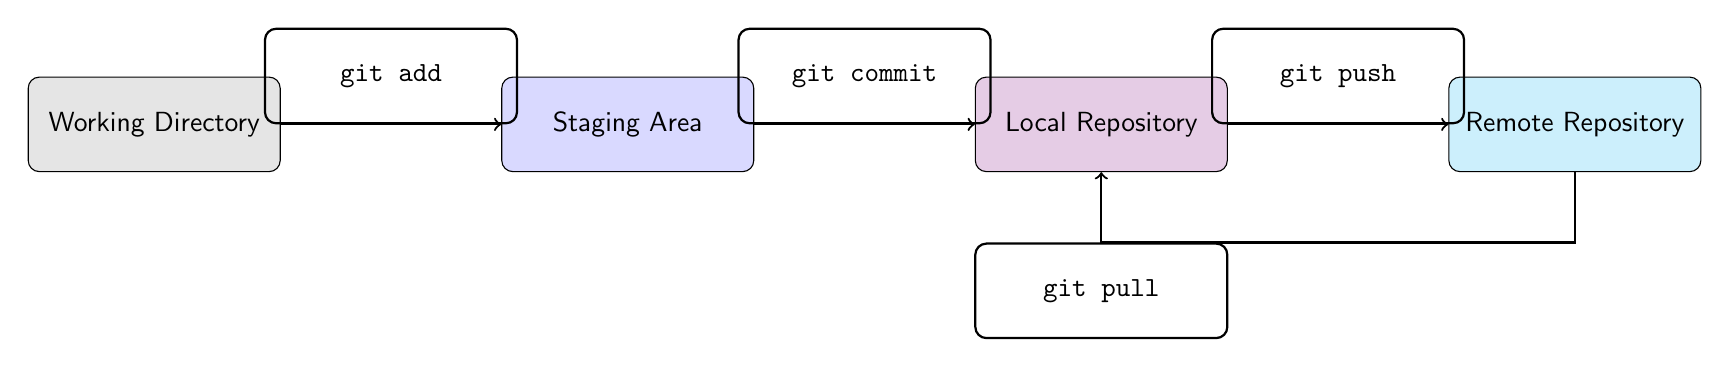
\begin{tikzpicture}[
    node distance=2.5cm and 2.8cm,
    every node/.style={rectangle, draw, rounded corners, minimum height=1.2cm, minimum width=3.2cm, font=\sffamily},
    arrow/.style={->, thick}
]

% Nodes
\node (wd)    [fill=gray!20]                  {Working Directory};
\node (stg)   [fill=blue!15, right=of wd]     {Staging Area};
\node (local) [fill=violet!20, right=of stg]  {Local Repository};
\node (remote)[fill=cyan!20, right=of local]  {Remote Repository};

% Arrows
\draw[arrow] (wd) -- node[above]{\texttt{git add}} (stg);
\draw[arrow] (stg) -- node[above]{\texttt{git commit}} (local);
\draw[arrow] (local) -- node[above]{\texttt{git push}} (remote);
\draw[arrow] (remote) -- ++(0,-1.5) -| node[below]{\texttt{git pull}} (local);

\end{tikzpicture}
}
\end{center}

This lifecycle ensures changes are intentionally managed at each step, promoting a clear separation between uncommitted, committed, and shared code states.

\subsection{Fundamental Git Commands}

This section outlines the most commonly used Git commands for managing source code, tracking changes, and collaborating with remote repositories. These commands form the foundation of most Git workflows.

\subsubsection{Initialising a Repository}

To create a new Git repository in the current directory:

\begin{minted}[fontsize=\small]{bash}
git init
\end{minted}

\noindent This sets up a new local repository by creating a \texttt{.git} directory containing all version control metadata.

\subsubsection{Cloning a Repository}

To create a local copy of an existing remote repository:

\begin{minted}[fontsize=\small]{bash}
git clone https://github.com/example/project.git
\end{minted}

\noindent This creates a local folder containing the entire commit history and working directory from the remote source.

\subsubsection{Checking Repository Status}

To check which files have been modified, staged, or remain untracked:

\begin{minted}[fontsize=\small]{bash}
git status
\end{minted}

\noindent This is useful before staging or committing to verify the current state of the working directory.

\subsubsection{Staging Changes}

To stage a file for commit:

\begin{minted}[fontsize=\small]{bash}
git add filename.java
\end{minted}

\noindent To stage all changes in the current directory:

\begin{minted}[fontsize=\small]{bash}
git add .
\end{minted}

\noindent Staged files are added to the index (staging area) and will be included in the next commit.

\subsubsection{Committing Changes}

To create a snapshot of staged changes:

\begin{minted}[fontsize=\small]{bash}
git commit -m "Add user authentication module"
\end{minted}

\noindent This saves the changes to the local repository history with a message describing the update.

\subsubsection{Viewing Commit History}

To view the list of previous commits:

\begin{minted}[fontsize=\small]{bash}
git log
\end{minted}

\noindent To view a more concise summary:

\begin{minted}[fontsize=\small]{bash}
git log --oneline
\end{minted}

\subsubsection{Inspecting Differences}

To view the changes in modified files (compared to last commit):

\begin{minted}[fontsize=\small]{bash}
git diff
\end{minted}

\noindent To compare staged changes to the last commit:

\begin{minted}[fontsize=\small]{bash}
git diff --cached
\end{minted}

\subsubsection{Pushing to a Remote Repository}

To upload local commits to the remote repository:

\begin{minted}[fontsize=\small]{bash}
git push origin main
\end{minted}

\noindent This updates the remote’s \texttt{main} branch with all commits from the local repository.

\subsubsection{Pulling from a Remote Repository}

To fetch and merge changes from the remote:

\begin{minted}[fontsize=\small]{bash}
git pull origin main
\end{minted}

\noindent This ensures the local branch is up to date with the remote.

\subsubsection{Creating and Switching Branches}

To create a new branch:

\begin{minted}[fontsize=\small]{bash}
git branch feature-login
\end{minted}

\noindent To switch to that branch:

\begin{minted}[fontsize=\small]{bash}
git checkout feature-login
\end{minted}

\noindent To create and switch in one step:

\begin{minted}[fontsize=\small]{bash}
git checkout -b feature-login
\end{minted}

\subsubsection{Checking Branches}

To list all local branches:

\begin{minted}[fontsize=\small]{bash}
git branch
\end{minted}

\noindent To list local and remote branches:

\begin{minted}[fontsize=\small]{bash}
git branch -a
\end{minted}

\subsubsection{Origin}

The term \texttt{origin} is a conventional name used to refer to the remote repository that a local repository is connected to. This association allows developers to push and pull updates with ease.

\begin{itemize}
    \item The name \texttt{origin} is automatically assigned when a repository is cloned.
    \item If the local repository was not cloned, the remote must be manually added using the following command:
\end{itemize}

\begin{minted}[fontsize=\small]{bash}
git remote add origin https://github.com/yourusername/your-repositoryname
\end{minted}

\noindent Once added, the remote repository can be referenced using \texttt{origin} in future commands such as \texttt{git push origin main} or \texttt{git pull origin main}. This configuration only needs to be performed once.




\subsection{JavaFx \& the Graphical User Interface (GUI)}

\subsection{The Integrated Build \& Javadoc}

\subsection{Refactoring \& Design Patterns}

\subsection{Threading and APIs}

% ===================================================================================
\newpage
\section{Software Development}

\subsection{Collaborative Programming \& High Performing Teams}

\subsection{Agile \& Sprint Planning}

\subsection{Persistence}

\subsection{Test Driven Development}

\subsection{User Testing}


\end{document}
